\documentclass[11pt]{beamer}
\beamertemplatenavigationsymbolsempty
\setbeamertemplate{footline}[frame number]
\usefonttheme[onlymath]{serif}



\makeatletter
\newlength\beamerleftmargin
\setlength\beamerleftmargin{\Gm@lmargin}
\makeatother

\usepackage{tikz}   
\usepackage[utf8]{inputenc}
\usepackage[english]{babel}
\usepackage[absolute,overlay]{textpos}
\usepackage{amsmath}
\usepackage{amsfonts}
\usepackage{amssymb}
\usepackage{graphicx}
%\usepackage{unicode-math}
\usepackage{multirow}
\usepackage{pbox}
\usepackage{array}
\usepackage{comment}

\usetheme{Warsaw}

\newcommand{\norm}[1]{\left\lVert#1\right\rVert}
\newcommand{\normsq}[1]{\left\lVert#1\right\rVert^2}
\setbeamercolor{framesource}{fg=gray}
\setbeamerfont{framesource}{size=\tiny}

\newcommand{\MX}{\mathbf{X}} %uncentered data
\newcommand{\MC}{\mathbf{C}} %centering
\newcommand{\MY}{\mathbf{Y}} %centered data
\newcommand{\MF}{\mathbf{F}_2} %F2-distance matrix
\newcommand{\MFT}{\mathbf{F}_3} %F3-distance matrix
\newcommand{\MP}{\mathbf{P}} % PCs
\newcommand{\ML}{\mathbf{L}} % loadings
\newcommand{\MK}{\mathbf{K}} % Kernel
\newcommand{\MSINGULAR}{\mathbf{\Sigma}} % Singular values matrix
\newcommand{\MEIGEN}{\mathbf{\Lambda}} % Eigenvalue matrix

\newcommand{\MEAN}{\boldsymbol{\mu}} % Kernel

\newcommand{\POP}[1]{X_{#1}}
\newcommand{\POPX}{\POP{X}}
\newcommand{\POPA}{\POP{A}}
\newcommand{\POPO}{\POP{O}}
\newcommand{\q}[1]{\hat{p}_{#1}}
\newcommand{\HAP}[1]{I_{#1}}
\newcommand{\HET}[1]{H_{#1}}
%\newcommand{\PCOAL}[2]{c_{#1\downarrow #2}}
\newcommand{\PCOAL}[2]{f}
\newcommand{\FX}[1]{F_{#1}}



\newcommand{\source}[1]{\begin{textblock*}{4cm}(8.7cm,8.6cm)
		\begin{beamercolorbox}[ht=0.5cm,right]{framesource}
			\usebeamerfont{framesource}\usebeamercolor[fg]{framesource} {#1}
		\end{beamercolorbox}
\end{textblock*}}


\begin{document}
	\author{Benjamin Peter}
	\title[PCA and F-stats]{Connections between $F$-statistics and Principal Component Analysis}
	
	%\subtitle{}
	%\logo{}
	%\institute{}
	%\date{}
	%\subject{}
	%\setbeamercovered{transparent}
	%\setbeamertemplate{navigation symbols}{}
	\begin{frame}[plain]
	\maketitle
\end{frame}

\begin{comment}
{
\usebackgroundtemplate{\includegraphics[width=1.4\paperwidth]{figures/bjorklund_art.jpeg}}%
\begin{frame}
	%\frametitle{bla}
	\source{@tombjorklund}
\end{frame}
}
\end{comment}


\begin{comment}


\begin{frame}
\frametitle{Population structure and ancient DNA}
\begin{center}
		\hspace*{-1.8\beamerleftmargin}
		\includegraphics<1>[width=\textwidth]{data/figures/ancient_dna_by_year.png}
		\includegraphics<2>[width=1.05\paperwidth]{data/figures/ancient_dna_map.png}		
\end{center}
		 \source{\url{https://reich.hms.harvard.edu/}}
\end{frame}

\begin{frame}[plain,c]
\begin{center}
	\Huge Conceptualizing Complex Population Structure remains a major challenge
\end{center}
\end{frame}
\end{comment}

\begin{frame}{Example: Map}
\includegraphics[width=\textwidth]{figures/sikora2019_fig1ab.png}
\source{Sikora et al. 2019}
\end{frame}

\begin{frame}{Example: PCA}
\includegraphics[width=.8\textwidth]{figures/sikora2019fig1c.png}
	\source{Sikora et al. 2019}
\end{frame}

\begin{frame}{Example: F-statistics}
\includegraphics[width=1.1\textwidth]{figures/sikora20019fige3.png}
	\source{Sikora et al. 2019}
\end{frame}

\begin{frame}{Example: Map}
	\includegraphics[width=\textwidth]{figures/hajdinjak2021fig1.png}
	\source{Hajdinjak et al. 2021}
\end{frame}

\begin{frame}{Example: PCA}
	\includegraphics[width=.8\textwidth]{figures/hajdinjak2021fige2.png}
	\source{Hajdinjak et al. 2021}
\end{frame}

\begin{frame}{Example: F-statistics}
	\begin{center}
	\includegraphics[width=.6\textwidth]{figures/hajdinjak2021fig2.png}	
	\end{center}
	
	\source{Hajdinjak et al. 2021}
\end{frame}



\begin{frame}
\frametitle{Goals of this talk}
\begin{itemize}
	\item Establish conceptual links between frameworks
	\begin{enumerate}
		\item How can we interpret PCA in context of $F$-stats?
		\item How can we interpret $F$-stats in the context of PCA?		
	\end{enumerate}
	\item (Use established links to improve data interpretation)
\end{itemize}
\only<2>{
\begin{alertblock}{Focus on intuition}
	Details in terms of estimation, normalization, missing data will be glossed over
\end{alertblock}
}
\end{frame}

\begin{frame}
	\frametitle{F-statistics: Trees vs. Admixture Graphs}
	\begin{columns}
		\begin{column}{0.5\textwidth}
			\includegraphics<1-2>[width=\textwidth]{figures/tree_intro.pdf}
			\includegraphics<3>[width=\textwidth]{figures/f2_intro.pdf}			
		\end{column}
	\begin{column}{0.5\textwidth}
		\includegraphics<2->[width=\textwidth]{figures/admixture_graph_intro.pdf}
	\end{column}
	
	\end{columns}
\end{frame}



\begin{frame}
\frametitle{$F$-statistics}
  \begin{tabular} {m{8.5cm}  |m{2cm}  }
	Definition & Branch length \\%& Path  \\
	\hline
	\vspace{6pt}$$\FX2(\POP1,\POP2) = \sum_l (X_{il} - X_{jl})^2 $$
	&\vspace{6pt}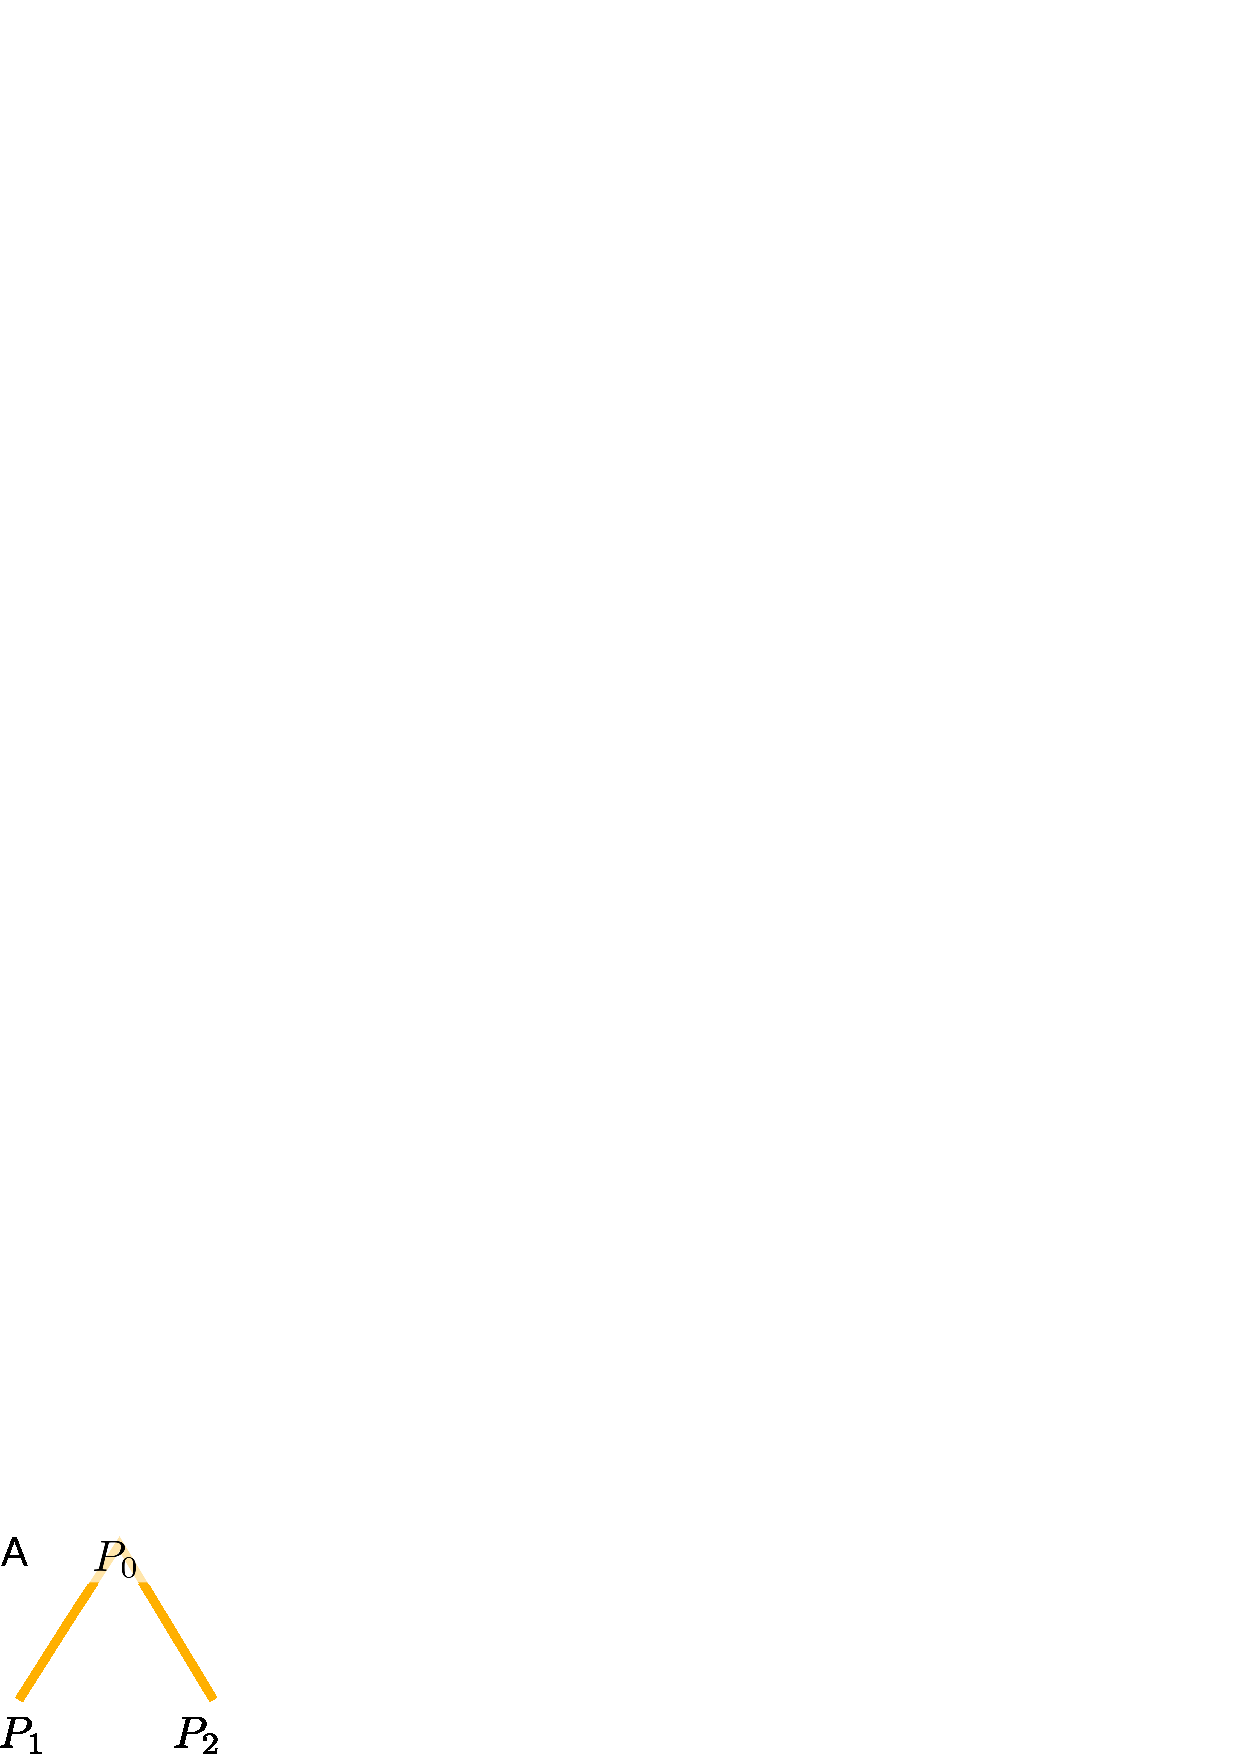
\includegraphics[scale=0.4]{figures/f2_internal.pdf}        
	%&\vspace{6pt}\includegraphics[scale=0.5]{./f2_admixture.eps}        
	\\ 
	\hline
	 \only<2->{\small{$$\FX3(\POP{x}; \POP1, \POP2) = \sum_l(X_{xl} - X_{1l})(X_{xl} - X_{2l}) $$}
	&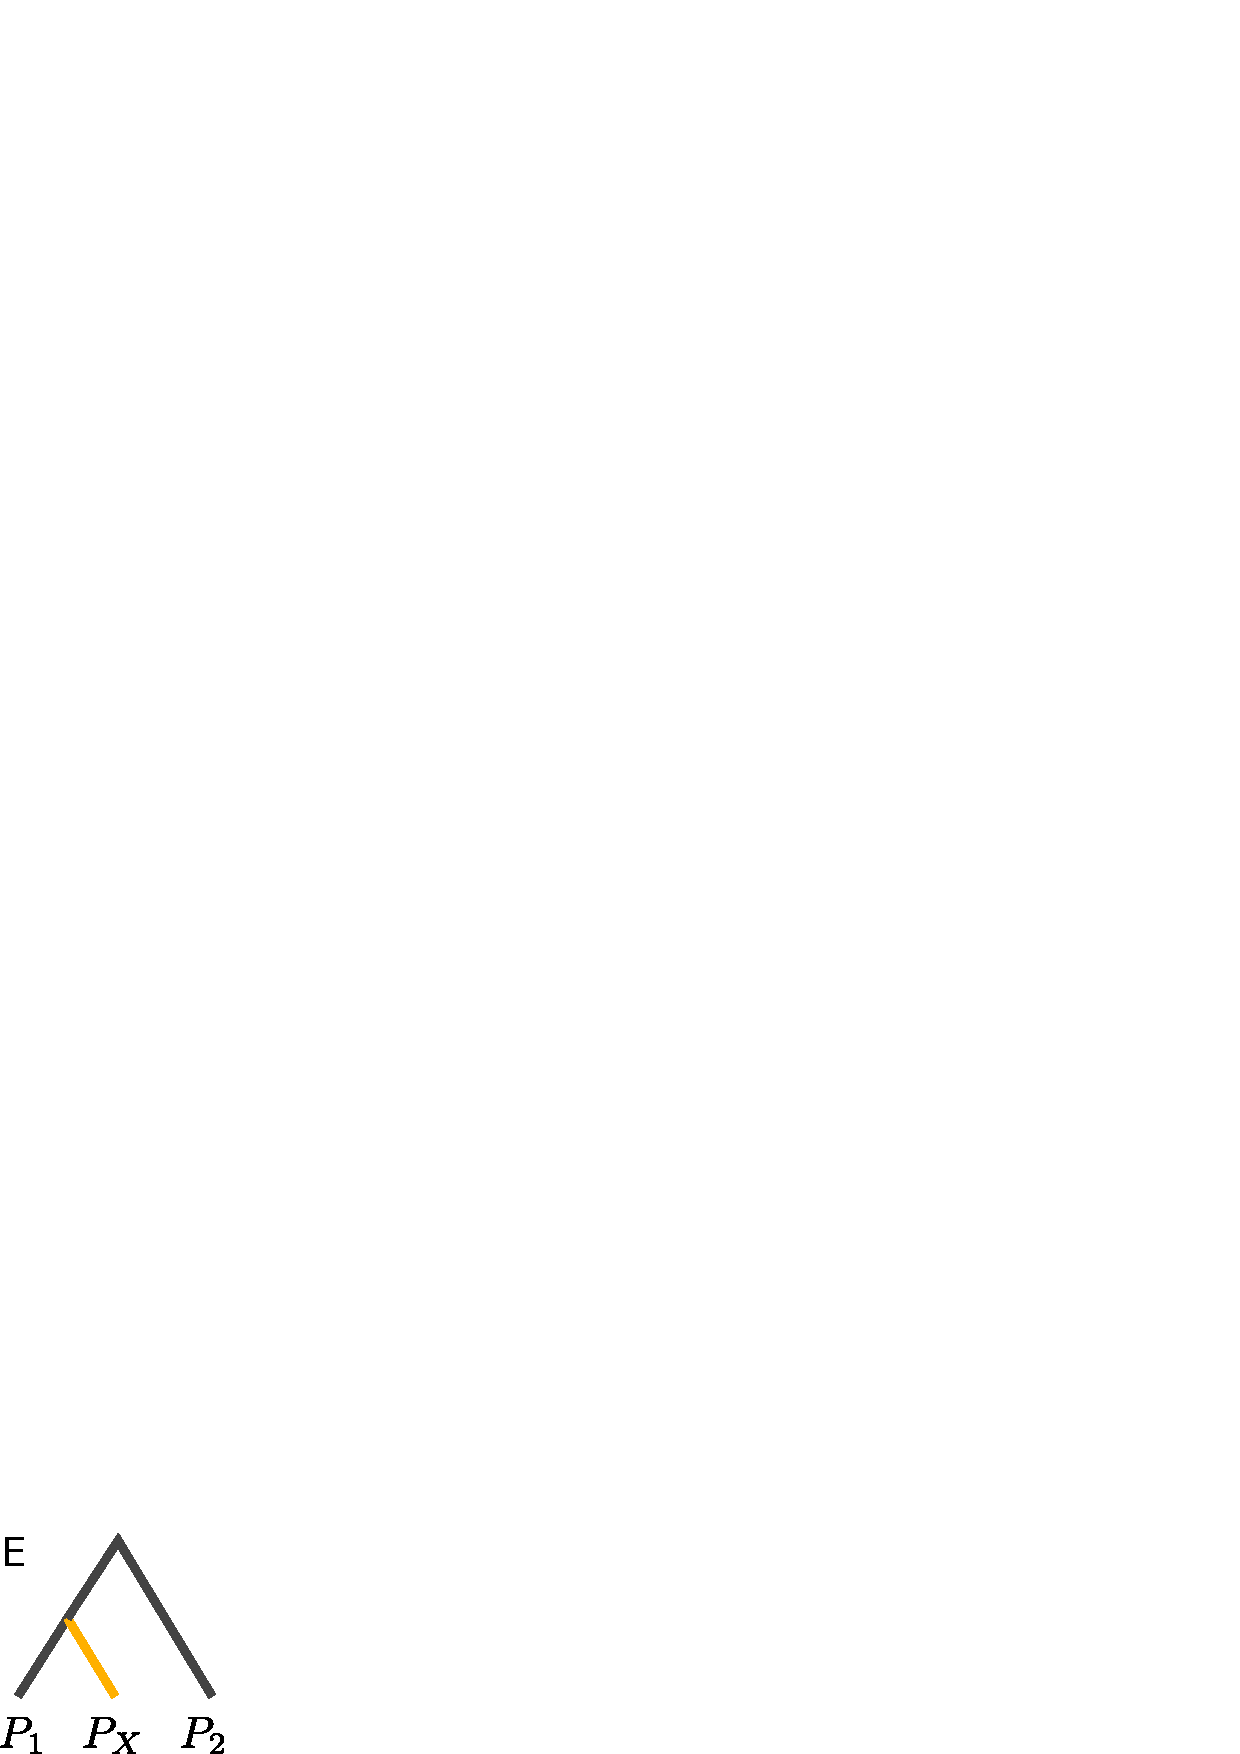
\includegraphics[scale=0.4]{figures//f3_internal.pdf}       
	%&\vspace{6pt}\includegraphics[scale=0.5]{./f3_admixture.eps}        
	\\ 
	\hline}
\only<3>{``Admixture''-$F_3$-statistic: If data is generated by a tree-like relationship, $F_3(P_X; P_1, P_2) \geq 0$
	&\vspace{6pt}\includegraphics[scale=0.4]{figures//f3_admixture.pdf}      
	\\ 
	\hline
}
\only<4>{``Outgroup''-$F_3$-statistic: Most similar pops have highest $F_3(P_2; P_X, P_1)$
	&\vspace{6pt}\includegraphics[scale=0.4]{figures//f3_outgroup.pdf}      
	\\ 
	\hline
}
	\only<5>{$$\FX4^{(B)}(\POP1; \POP2; \POP3, \POP4) = \sum_l(X_{1l} - X_{3l})(X_{2l} - X_{4l})$$
	&\vspace{6pt}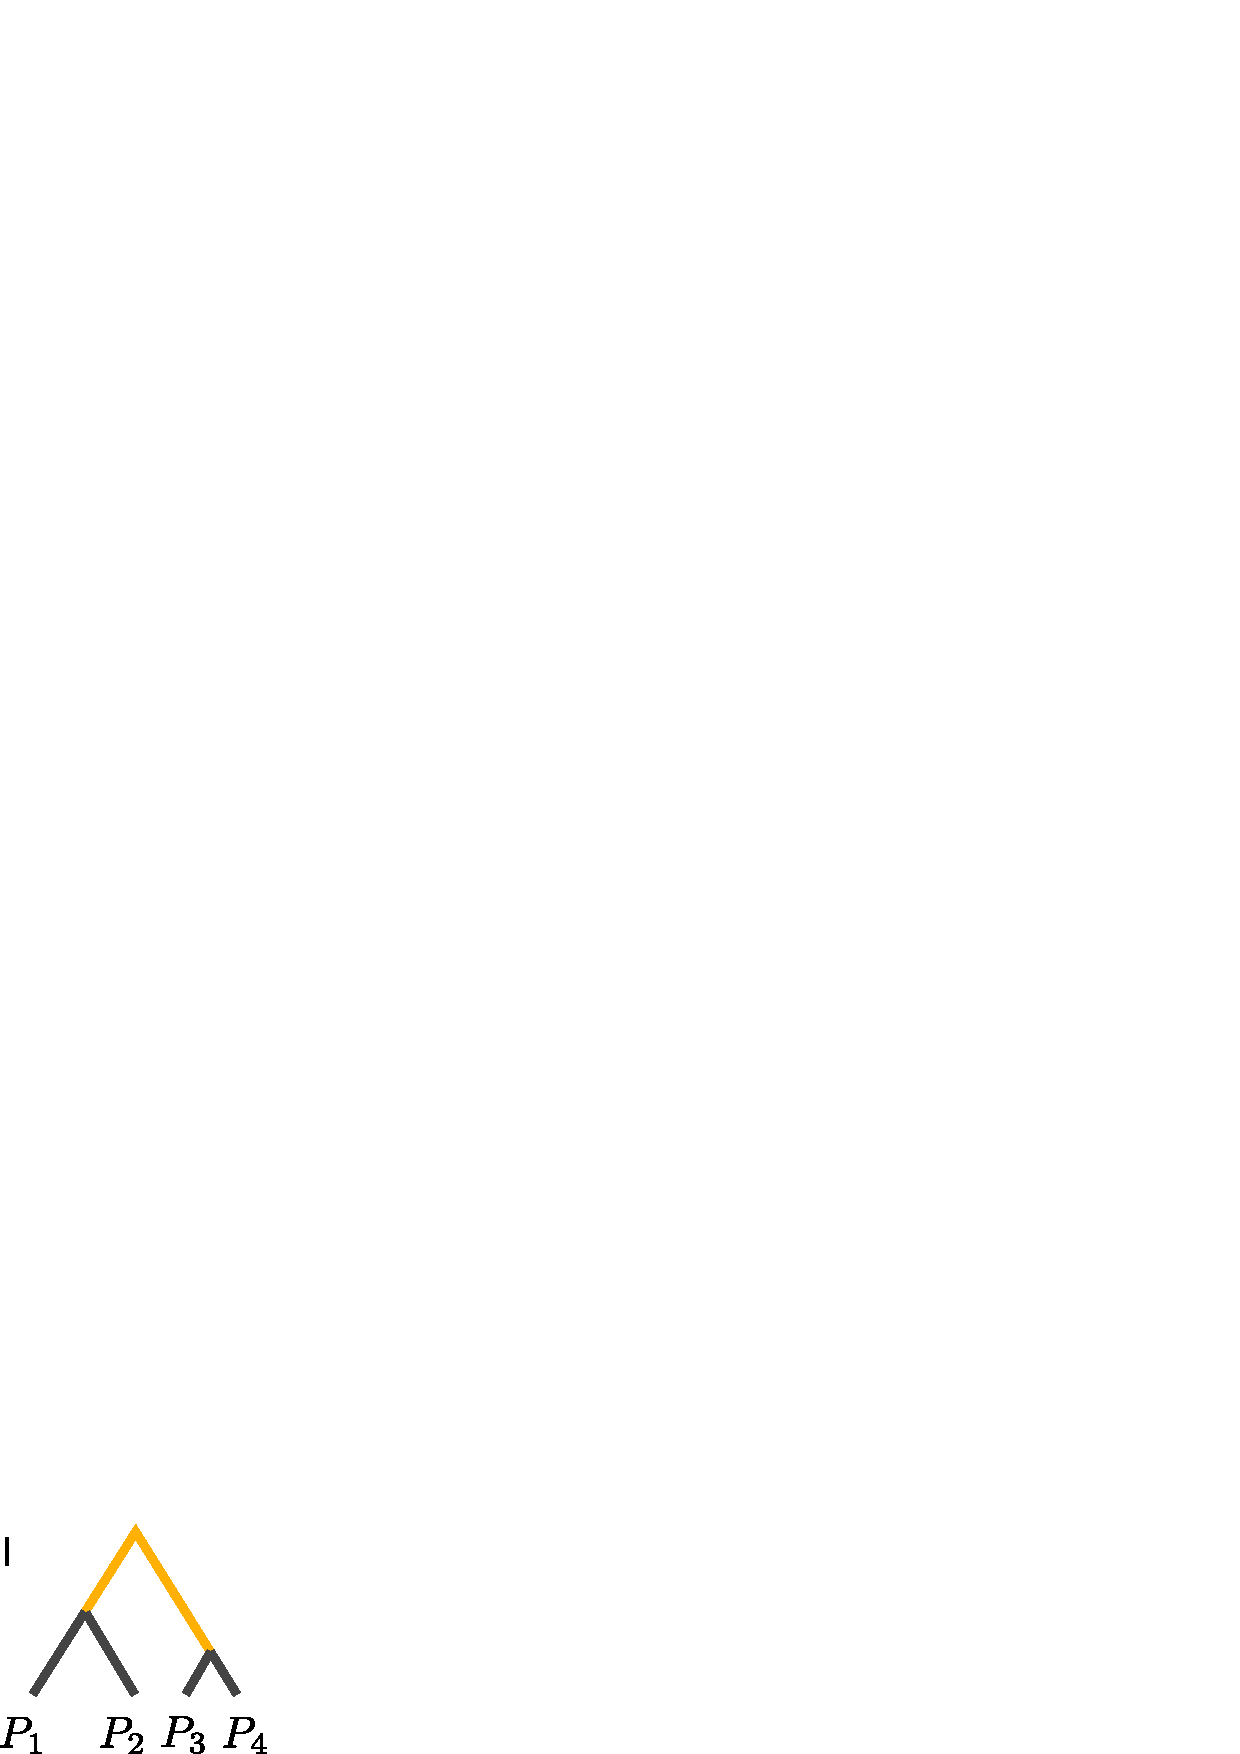
\includegraphics[scale=0.4]{figures//f4_internal_branch.pdf}        
	%&\vspace{6pt}\includegraphics[scale=0.5]{./f4b_admixture.pdf}        
	\\ 
	\hline
	}
	\only<6>{
	$$\FX4^{(T)}(\POP1; \POP2; \POP3, \POP4) = \sum_l(X_{1l} - X_{2l})(X_{3l} - X_{4l})$$
	&\vspace{6pt}\includegraphics[scale=0.4]{figures//f4_internal.pdf}        
	%&\vspace{6pt}\includegraphics[scale=0.5]{./f4_admixture.eps} \\ 
}
\end{tabular}

		\source{Patterson et al. 2012; Peter 2016}

\end{frame}


\begin{comment}
\begin{frame}
\frametitle{Principal Component Analysis}
\begin{columns}
	\begin{column}{0.5\textwidth}
		\includegraphics[width=1.1\textwidth]{figures/hajdinjak2021_fige2_no_legend.png}
	\end{column}
	\begin{column}{0.5\textwidth}
		\includegraphics<2>[width=1\textwidth]{figures/mcvean2009_fig3a.png}			
		\includegraphics<3->[width=1\textwidth]{figures/mcvean2009_fig3ab.png}		
		\includegraphics<4->[width=1\textwidth]{figures/mcvean2009_fig4b.png}
		\source{McVean, 2009}
	\end{column}
\end{columns}
\end{frame}
\end{comment}
	\begin{frame}
\frametitle{Principal Component Analysis}
	\begin{center}
		\includegraphics<1>{figures/pca1.pdf}
		\includegraphics<2>{figures/pca2.pdf}
		\includegraphics<3>{figures/pca3.pdf}
		\includegraphics<4>{figures/pca4.pdf}
		\includegraphics<5->{figures/pca5.pdf}						
		%\includegraphics<6>{figures/pca6.pdf}						
	\end{center}
\end{frame}


\begin{comment}
\begin{frame}
\frametitle{How to find PCs}
\begin{columns}
\begin{column}{0.4\textwidth}
	\includegraphics[width=\textwidth]{figures/pca3.pdf}
\end{column}
\begin{column}{0.7\textwidth}
	\begin{itemize}
		\item<1-> Singular Value Decomposition: $\MY = (\mathbf{U}\mathbf{D})\mathbf{L} = \mathbf{P}\mathbf{L}$
		\item<2-> Eigendecomposition of $\MY\MY^T$: $\MY\MY^T = \mathbf{U}\mathbf{D}^2\mathbf{U}^T = \MP\MP^T$
		\only<3>{\item $(\MY\MY^T)_{ij}$}
		\item<4-> $(\MY\MY^T)_{ij} = \sum_l (x_{il} - \mu_l)(x_{jl} - \mu_l)$
		\item<5-> \small{$\FX3(\POP{x}; \POP1, \POP2) = \sum_l(X_{1l}-X_{xl})(X_{2l}-X_{xl})$}
		\item<6-> $(\MY\MY^T)_{ij} = F_3(\MEAN; \MX_i, \MX_j)$
	\end{itemize}
\end{column}			
\end{columns}
\vspace{30px}
\only<6>{
\begin{alertblock}{Observation}
	PCA is equivalent to outgroup-$F_3$-analysis with sample mean as outgroup
\end{alertblock}
}
\end{frame}
\end{comment}

\begin{frame}
\frametitle{(metric) Multi-Dimensional Scaling (MDS)}

\begin{columns}
\begin{column}{0.5\textwidth}
\includegraphics<1>{figures/pca1.pdf}
\includegraphics<2>{figures/mds1.pdf}
\includegraphics<3->{figures/mds2.pdf}
\end{column}
\begin{column}{0.5\textwidth}
\includegraphics<4>{figures/mds3.pdf}		
\includegraphics<5>{figures/mds4.pdf}		
\includegraphics<6>{figures/mds5.pdf}		
\includegraphics<7>{figures/mds6.pdf}					
\end{column}
\end{columns}
		\only<7->{
	\begin{alertblock}{Observation}
		MDS on $F_2$ is equivalent to PCA
\end{alertblock}}
\end{frame}

\begin{frame}
	\frametitle{Constructing PCA}
	Let $\MX$ be a matrix of genotypes, $\MC$ a centering matrix that subtracts row means and $\MY = \MC\MX$ be the centered genotype matrix, and $\MF$ be a matrix of $F_2$-statistics. 
	
	The following constructions of PCA are equivalent:
	\begin{itemize}
		\item Singular Value Decomposition of $\MY$
		\item Eigendecomposition of $\MY\MY^T$
		\item Eigendecomposition of $-\frac{1}{2}\MC\MF\MC$ 
	\end{itemize}
	\only<2->{
	\begin{alertblock}{Observation}
		$\MF$ is a sufficient statistic to compute a PCA
\end{alertblock}}
\end{frame}

\begin{comment}
\begin{frame}
\frametitle{PCA is MDS on $\MF$}

\begin{itemize}
\item<1-> PCA is decomposition of Covariance matrix: $\MY\MY^T$
\item<2-> Consider $\MF; f_{ij} = F_2(X_i, X_j) = \sum_l (X_{li}^2 -X_{lj})^2$
\item<3-> Consider $\MF; f_{ij} = \sum_l X_{li}^2 + \sum_l X_{lj}^2 - 2 \sum_l X_{li}X_{lj}$
\item<4-> MDS is Eigendecomposition of $-\frac{1}{2}\MC\MF\MC$
\only<5>{\item<5> $\MC\MF\MC = \MC\MX_i^2\MC + \MC\MX_j^2\MC - 2\MC\MX\MX^T\MC$}
\item<6-> $\MC\MF\MC = \underbrace{\MC\MX_i^2\MC}_{0}  + \underbrace{\MC\MX_j^2\MC}_{0} - 2\underbrace{\MC\MX\MX^T\MC}_{\MY\MY^T}$
\end{itemize}


\only<7>{
\begin{alertblock}{Observation}
PCA is equivalent to MDS on $\MF$
\end{alertblock}
}
\end{frame}



\begin{frame}
\frametitle{PCA is MDS on Outgroup$\MFT$}

\begin{itemize}
\item<1-> PCA is decomposition of Covariance matrix: $\MY\MY^T$
\item<2-> $\MFT(O); f_{ij} = F_3(O; X_i, X_j)$
\item<2-> $f_ij = \sum_l \big[ o_l^2 - o_l X_{li} - o_l X_{li} +  X_{li} X_{lj} \big]$
\item<3-> $\MC\MFT\MC = \underbrace{\MC O^2\MC}_{0}  - 
\underbrace{\MC O\MX_i\MC}_{0} -
\underbrace{\MC O\MX_j\MC}_{0} + 
\underbrace{\MC\MX\MX^T\MC}_{\MY\MY^T}$
\end{itemize}


\only<5>{
\begin{alertblock}{Observation}
Decomposition of \emph{any} centered $F_3$-matrix is equivalent to PCA.
\end{alertblock}
}
\end{frame}


\begin{frame}
\frametitle{0-diagonal MDS}
In aDNA applications (e.g. Fu et al 2016), MDS is performed on
\small{
$$\mathbf{M} = 
\begin{pmatrix}
0                     & 1 - f_3(O; X_1, X_2) & \dots & 1 - f_3(O; X_1, X_n)\\
 1 - f_3(O; X_1, X_2) & 0 &                    \dots & 1 - f_3(O; X_2, X_n)\\
 \vdots &             \vdots                 & \ddots& 1 - f_3(O; X_i, X_n)\\
 1 - f_3(O; X_1, X_n) & 1 - f_3(O; X_2, X_n)   & \dots & 0
\end{pmatrix}
$$}\source{Fu et al. 2016}
It can be shown that 
$$\MC\mathbf{M}\MC = \MC\MF\MC + \MC\mathbf{O}\MC$$
with $o_{ii} = f_2(O, X_i) - 1; o_{ij} = 0$
\end{frame}




\begin{frame}
\frametitle{How can we interpret PCA in context of $F$-stats?}
\begin{itemize}
	\item PCA is decomposition of $\MFT(\MEAN, X_1, X_2)$-matrix
	\item PCA is a function of (unnormalized)-$\MF$-matrix
	\begin{itemize}
		\item same information content
		\item differences in analysis choices (individual/population, normalization, estimate) need to be justified
	\end{itemize}
	\item<2-> setting diagonal allows some leeway
	\item<3-> \emph{Conjecture}: PCA is analogous to midpoint-rooted phylogenetic analyses; Outgroup-$F_3$ allow other rootings.

	
\end{itemize}
\end{frame}
\end{comment}

\begin{frame}
	\frametitle{Geometric Interpretation}
	\includegraphics[width=\textwidth]{figures/oteo_header.png}

	\begin{columns}
		\begin{column}{.4\textwidth}
	   \includegraphics<2->[width=\textwidth]{figures/oteo_fig1a.png}
		\end{column}
	\begin{column}{.6\textwidth}

	\only<2>{\begin{align*}
	F_2(X_1, X_2) &= \sum_l (X_{1l} - X_{2l})^2\\
	F_3(X_1; X_2, X_3) &= \sum_l (X_{1l} - X_{2l})(X_{1l}-X_{13})\\
	F_4(X_1, X_2; X_3, X_4) &= \sum_l (X_{1l} - X_{2l})(X_{3l}-X_{4l})
	\end{align*}}
	\only<3->{\begin{align*}
	F_2(X_1, X_2) &= \normsq{X_{1l} - X_{2l}}\\
	F_3(X_1; X_2, X_3) &= \langle X_1 - X_2, X_1 - X_3\rangle\\
	F_4(X_1, X_2; X_3, X_4) &= \langle X_1 - X_2, X_3 - X_4\rangle\end{align*}}
\end{column}	
\end{columns}
\only<4->{
	\begin{alertblock}{Interpretation}
		Think of $F$-statistics as inner products in L-dimensional \emph{data space}.
	\end{alertblock}
}
\end{frame}

\begin{frame}
\frametitle{$F$-statistics on PCA-plot}
\begin{itemize}
	\item Recall that PCA is just rotation around centroid
	\item<3-> Distances (such as $F_2$) are invariant to  rotation
\end{itemize}
\begin{center}
	\includegraphics<2>{figures/pca2.pdf}
	\includegraphics<2>{figures/pca4.pdf}						
\end{center}
\begin{itemize}
	\item<4-> $$F_2(X_1, X_2) = \sum_{\text{loci}}(x_{1l} - x_{2l})^2$$
	\item<5-> $$F_2(X_1, X_2) = \sum_{\text{PCs}}(x_{1p} - x_{2p})^2$$	
\end{itemize}
\only<6->{
	\begin{alertblock}{Observation}
		$F_2$ can be decomposed into contributions from different principal components
	\end{alertblock}
}
\end{frame}


\begin{frame}
\frametitle{$F$-statistics on PCA-plot}
\begin{columns}
	\begin{column}{0.5\textwidth}
		\includegraphics<1>{figures/pca1.pdf}
		\includegraphics<2->{figures/pca1b.pdf}		
	\end{column}
	\begin{column}{0.5\textwidth}
		\begin{itemize}
			\item<3-> $F$-statistics have a geometrical representation on PCA-plot
			\item<3-> Exact only if we use \emph{all} PCs
			\item<4-> If first two PCs capture relevant population structure, $F$-statistics will be well approximated
		\end{itemize}		
	\end{column}
\end{columns}
\end{frame}

\begin{frame}
	\frametitle{Technical interlude: Does PCA provide a good approximation?}
	\pause
	\begin{align*}
	F_2(P_i, P_j) &= \sum_{k=1}^K(p_{ik} - p_{jk})^2 &+ \sum_{k=K+1}^n(p_{ik} - p_{jk})^2\nonumber\pause\\
	&= {\hat{F_2}^{(K)}(P_i, P_j)} &+ {\epsilon^{(K)}(P_i, P_j)}
	\end{align*}
	\pause
	The total error is then
	\begin{equation}
	\sum_{i,j} \epsilon^{(K)}(P_i, P_j)^2 = \sum_{i,j} \left(\hat{F_2}^{(K)}(P_i, P_j) - F_2^{(K)}(P_i, P_j)\right)^2 = \normsq{\MF - \hat{\MF}}_F \text{,}
	\end{equation}\pause
	\begin{alertblock}{Observation}
		$\hat{F}_2$ provides optimal approximation in the sense that total squared error between \emph{all} $F_2$-statistics is minimized.
	\end{alertblock}
\end{frame}

\begin{frame}
	\frametitle{Technical interlude 2: What about projections?}
	Recall that the basic way we project a sample onto a PCA is by multiplying with $\ML$
	\begin{align*}
	F_2(X_i, X_{\text{new}}) &= F_2(Y_i, Y_{\text{new}})\nonumber\\ 
	&= F_2(P_i, P_{\text{proj}}) + F_2(P_{\text{proj}}\ML, Y_{\text{new}})\nonumber\pause\\
	&= \hat{F_2}(P_i, P_j) + {\epsilon(P_i, P_j)} + F_2(P_{\text{proj}}\ML, Y_{\text{new}}) \label{eq:approx}.
	\end{align*}
	\pause
	\begin{alertblock}{Observation}
		Projections adds another error-term that will be small if the projected sample is well-represented by variation of reference sample.
	\end{alertblock}
\end{frame}

\begin{frame}
	\frametitle{Global Data}
	\includegraphics[width=\paperwidth]{data/figures/sample_map_world.png}
\end{frame}
\begin{frame}
	\frametitle{Global PCA}
	\begin{center}
		\begin{tikzpicture}
		\node (img1) {\includegraphics[height=5cm]{data/figures/talk/world_pca.png}};
		\node (img2) at (img1.south)[yshift=-1.1cm] {\includegraphics[height=5cm]{data/figures/sample_map_world2.png}};
		\end{tikzpicture}		
	\end{center}
\end{frame}
\begin{frame}
	\frametitle{Westeurasian Data}
	\includegraphics{data/figures/sample_map_eu.png}
\end{frame}

\begin{frame}
	\frametitle{Westeurasian PCA}
\begin{tikzpicture}
\node (img1)[xshift=-1cm] {\includegraphics[height=6cm]{data/figures/talk/eu_pca.png}};
\node (img2) at (img1.south east)[yshift=-1.1cm] {\includegraphics[height=5cm]{data/figures/sample_map_eu2.png}};
\end{tikzpicture}	
\end{frame}





\begin{frame}
\frametitle{$F_2$-statistic on PCA-plot}
\begin{columns}
	\begin{column}{0.5\textwidth}
		\includegraphics<1>{figures/f3_on_pca_1b.pdf}
		\includegraphics<2>{figures/f2_on_pca.pdf}
	\end{column}
	\begin{column}{0.6\textwidth}
		\begin{itemize}
			\item $F_2(X_1, X_2) = \sum_l(X_{1l}-X_{2l})^2$
			\item $F_2(X_1, X_2) = \normsq{X_1 -  X_2}$			
		\end{itemize}		
	\end{column}
\end{columns}
\end{frame}

\begin{frame}
	\frametitle{Distance from Sardinians}
	\begin{center}
		\begin{tikzpicture}
		\node (img1) {\includegraphics[height=5cm]{data/figures/talk/world_pca_highlightf2.png}};
		\node (img2) at (img1.south)[yshift=-1.1cm] {\includegraphics[height=5cm]{data/figures/sample_map_world2.png}};\pause
		\node (img3) at (img1.west)[xshift=-1cm] {\includegraphics[height=6cm]{data/figures/talk/world_f2.png}};
		\end{tikzpicture}		
	\end{center}
\end{frame}



\begin{frame}
\frametitle{Admixed populations ($F_3$) on PCA-plot}
\begin{columns}
	\begin{column}{0.4\textwidth}
		\includegraphics<1>{figures/f3_on_pca_1b.pdf}
		\includegraphics<2-4>{figures/f3_on_pca_1.pdf}		
		\includegraphics<5>{figures/f3_on_pca_1d.pdf}				
	\end{column}
	\begin{column}{0.6\textwidth}
		\begin{itemize}
			\item<1-> Given $X_1, X_2$, which pops have $F_3 < 0$?	
			\item<2-> $F_3(Y; X_1, X_2) = 0$ is a circle!
%			\item<3-> Samples outside circle will always have positive $F_3$
			\item<5> Circle is larger when considering more PCs
		\end{itemize}
	
	\only<1>{\begin{center}
			\includegraphics[scale=1]{figures//f3_admixture.pdf}
		\end{center}}  		
		\includegraphics<4>[width=\textwidth]{figures/mcvean2009_fig4b.png}
	\end{column}
\end{columns}
\end{frame}

\begin{frame}
	\frametitle{Westeurasian PCA}
	\begin{tikzpicture}
	\node (img1)[xshift=-1cm] {\includegraphics[height=6cm]{data/figures/talk/eu_pca.png}};
	\node (img2) at (img1.south east)[yshift=-1.1cm] {\includegraphics[height=5cm]{data/figures/sample_map_eu2.png}};
	\end{tikzpicture}	
\end{frame}
\begin{frame}
	\frametitle{Westeurasian PCA}
	\begin{tikzpicture}
	\node (img1)[xshift=-1cm] {\includegraphics[height=6cm]{data/figures/talk/eu_pca_f3.png}};
	\node (img2) at (img1.south east)[yshift=-1.1cm] {\includegraphics[height=5cm]{data/figures/sample_map_eu_f3.png}};
	\end{tikzpicture}	
\end{frame}

\begin{frame}
	\frametitle{Westeurasian PCA}
	\begin{tikzpicture}
	\node (img1)[xshift=-1cm] {\includegraphics[height=6cm]{data/figures/talk/eu_pca_f32.png}};
	\node (img2) at (img1.south east)[yshift=-1.1cm] {\includegraphics[height=5cm]{data/figures/sample_map_eu_f3.png}};
	\end{tikzpicture}	
\end{frame}

\begin{frame}
\frametitle{Summary Admixture $F_3$}
\begin{columns}
	\begin{column}{.5\textwidth}
\begin{enumerate}[<+->]
	\item $F_3 < 0 \Leftrightarrow $ $n$-ball on PCA
	\item on 2D-plot samples might be in circle, but positive $F_3$
	\item Samples outside circle always have $F_3 > 0$ 
	
\end{enumerate}
	\end{column}
	\begin{column}{.7\textwidth}
\includegraphics[width=\textwidth]{data/figures/talk/eu_pca_f32.png}
\end{column}
\end{columns}

\end{frame}



\begin{comment}
\begin{frame}
\frametitle{Admixture $F_3$-stats on PCA-plot}
\begin{columns}
	\begin{column}{0.4\textwidth}
		\includegraphics<1>{figures/f3_on_pca_2b.pdf}
		\includegraphics<2->{figures/f3_on_pca_2.pdf}		
	\end{column}
	\begin{column}{0.6\textwidth}
		\begin{itemize}
			\item<1-> Given $X_1, X_x$, which pops $X_2$ have $F_3 < 0$?	
			\item<2-> $F_3$ is 0 if $(X_x; X_1), (X_x; X_2)$ form a right angle!
			\item<3-> Inner (dot) product: $F_3(X_x; X_1, X_2) = \langle X_x - X_1, X_x - X_2\rangle$
		\end{itemize}		
	\end{column}
\end{columns}
\end{frame}
\end{comment}

\begin{frame}
	\frametitle{Outgroup $F_3$-stats on PCA-plot}
	\begin{columns}
		\begin{column}{0.4\textwidth}
			\includegraphics<1-2>{figures/f3_on_pca_3b.pdf}
			\includegraphics<3>{figures/f3_on_pca_3.pdf}		
			\includegraphics<4->{figures/f3_on_pca_3c.pdf}			
		\end{column}
		\begin{column}{0.6\textwidth}
			\begin{itemize}
				\item<1-> Given $X_O, X_1$, which pop $X_2$ has highest $F_3$?
			\end{itemize}
		\only<1>{\begin{center}
				\includegraphics[scale=1]{figures/f3_outgroup.pdf}
		\end{center}}
		\begin{itemize}	
	\item<2-> As $F_3 = \langle X_O - X_1, X_O - X_2 \rangle$, project $\overline{X_OX_2}$ on $\overline{X_OX_1}$
	\item<3-> $F_3$ is proportional to segment in dir $X_0 \rightarrow X_1$
	\item<4-> Pop furthest on axis has highest $F_3$.
\end{itemize}		
	  	
		\end{column}
	\end{columns}
\end{frame}


\begin{frame}
\frametitle{$F_3$(Mbuti; Mozabite, X))}
\begin{center}
\begin{tikzpicture}
\node (img1) {\includegraphics[height=5cm]{data/figures/talk/world_pca.png}};
\node (img2) at (img1.south)[yshift=-1.1cm] {\includegraphics[height=5cm]{data/figures/sample_map_worldf32.png}};
\end{tikzpicture}
\end{center}
\end{frame}

\begin{frame}
	\frametitle{$F_3$(Mbuti; Mozabite, X))}
	\begin{center}
		\begin{tikzpicture}
		\node (img1) {\includegraphics[height=5cm]{data/figures/talk/world_pca2.png}};
		\node (img2) at (img1.south)[yshift=-1.1cm] {\includegraphics[height=5cm]{data/figures/sample_map_worldf3.png}};
		\end{tikzpicture}
	\end{center}
\end{frame}

\begin{frame}
	\frametitle{$F_3$(Mbuti; Mozabite, X))}
	\begin{center}
		\begin{tikzpicture}
		\node (img1) {\includegraphics[height=5cm]{data/figures/talk/world_pca3.png}};
		\node (img2) at (img1.south)[yshift=-1.1cm] {\includegraphics[height=5cm]{data/figures/sample_map_worldf3.png}};
		\end{tikzpicture}
	\end{center}
\end{frame}



\begin{frame}
	\frametitle{Outgroup-$F_3$}
	\begin{columns}
		\begin{column}{.5\textwidth}
			\includegraphics<1->[width=\textwidth]{data/figures/talk/outgroup_f31.png}
		\end{column}
		\begin{column}{.5\textwidth}
			\includegraphics<2->[width=\textwidth]{data/figures/talk/outgroup_f32.png}
		\end{column}
	\end{columns}
	\begin{itemize}
		\item <3-> Outgroup-$F_3$ corresponds to projection on axis from Outgroup to test population
		\item <4-> Two PCs give excellent approximation
		\item <5-> Offset by constant due to local population structure
	\end{itemize}
\end{frame}





\begin{frame}
\frametitle{ $F_4$-stats on PCA-plot}
\begin{columns}
	\begin{column}{0.4\textwidth}
		\includegraphics<1>{figures/f4_on_tree3.pdf}
		\includegraphics<2->{figures/f4_on_tree2.pdf}
	\end{column}
	\begin{column}{0.7\textwidth}
		\begin{itemize}
			\item<1-> $F_4(X_1, X_2 ; X_3, X_4)$ is internal branch of a tree
			\item<2> $F_4(X_1, X_2 ; X_3, X_4) \Leftrightarrow \langle X_1 - X_2; X_3 - X_4\rangle$			
			\item<2> $F_4$ is zero if $X_1 -X_2$ and $X_3 -X_4$  are orthogonal
		\end{itemize}	
	\end{column}
\end{columns}
\end{frame}

\begin{frame}
	\frametitle{ $F_4$-stats on PCA-plot}
	\begin{columns}
		\begin{column}{0.5\textwidth}
			\includegraphics{figures/f4_on_tree2.pdf}
		\end{column}
		\begin{column}{0.5\textwidth}	
			\includegraphics{figures/f4_on_pca2.pdf}	
		\end{column}
	\end{columns}
\end{frame}

\begin{frame}
	\frametitle{ $F_4$-stats on PCA-plot}
	\begin{columns}
		\begin{column}{0.5\textwidth}
			\includegraphics{figures/f4_on_tree2.pdf}
		\end{column}
		\begin{column}{0.5\textwidth}	
			\includegraphics{figures/f4_on_pca.pdf}	
		\end{column}
	\end{columns}
\begin{equation*}
\text{Cor}(X_1 - X_2, X_3 - X_4) =  \frac{\langle X_1 - X_2, X_3 - X_4 \rangle}{\norm{X_1-X_2}\norm{X_3-X_4}} = \cos(\phi),\label{eq:angle}
\end{equation*}
\end{frame}

\begin{frame}
	\frametitle{Two Gradients in Westeurasian PCA}
\begin{columns}
	\begin{column}{.7\textwidth}
		$$F_4(\text{Georgian}, \text{Saudi}; \text{Sardinian}, X)$$
\includegraphics<1-2>[width=\textwidth]{data/figures/talk/anglepca.png}
\includegraphics<3>[width=\textwidth]{data/figures/talk/anglepca13.png}
	\end{column}
	\begin{column}{.4\textwidth}
	\includegraphics<2->[width=\textwidth]{data/figures/talk/angle.pdf}
\end{column}
\end{columns}
\end{frame}




\begin{frame}
\frametitle{Where does Orthogonality come from?}
\begin{columns}
	\begin{column}{0.5\textwidth}
		\includegraphics<1->{figures/f3_nonorthogonal.pdf}
	\end{column}
	\begin{column}{0.5\textwidth}
		\includegraphics<2>{figures/f3_orthogonal.pdf}
	\end{column}
\end{columns}
\end{frame}





\begin{frame}
	\frametitle{How can we interpret $F$-stats in the context of PCA?}
	\begin{itemize}[<+->]
		\item $F$-stats have geometric interpretation that aide in interpretation of PCA
		\item Inconsistenty between $F$-stats and PCA hint at important structure in higher PCs
		\item exact in $n$-dimensional, approximate in 2D
		\item $F_3$ is a (hyper)-circle
		\item $F_4$ is angle and tests orthogonality on PCA
		\item Orthogonality stems from independence of drift in distinct parts of history
	\end{itemize}
\end{frame}



\begin{comment}
\begin{frame}
	\frametitle{Thank You!}
	\includegraphics[width=\textwidth]{figures/group_photo.png}
\end{frame}
\end{comment}


\end{document}